\documentclass[a4paper, 11pt]{article}
\usepackage[utf8]{inputenc}
\usepackage[T1]{fontenc}
\usepackage{lmodern}
\usepackage{titlesec}
\usepackage{tikz}
\usepackage[left=1.5cm, top=2cm, right=2.5cm]{geometry}
\usepackage{float}

\titleformat*{\section}{\sffamily\Large\bfseries}
\titleformat*{\subsection}{\sffamily\large\bfseries}
\titleformat*{\subsubsection}{\sffamily\normalsize\bfseries}
\titleformat*{\paragraph}{\sffamily\normalsize\bfseries}

\begin{document}

\section*{Persistence of Vision Display - Acceleration model}
In order to display the correct column of the desired image, the persistence of vision (POV) display has to be aware of its position in the direction it is moved in. Assuming the display is manually shaked by a human, we can make some assumptions on the type of movement it performs. Namely, acceleration measurements show that the device is usually swiped with a motion that can be approximated by linearly increasing / decreasing acceleration, thus piecewise constant jerk as shown in figure \ref{fig:acc}.

\begin{figure}
	\centering
	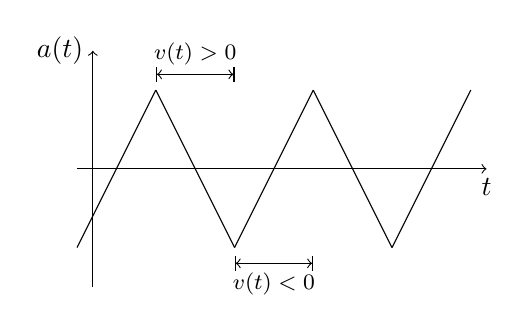
\begin{tikzpicture}
		\draw[->] (-0.2, 1.5) -- (5, 1.5) node[below] {$t$};
		\draw[->] (0, 0) -- (0, 3) node[left] {$a(t)$};

		\draw[-] (-0.2, 0.5) -- (0.8, 2.5);
		\draw[-] (0.8, 2.5) -- (1.8, 0.5);
		\draw[-] (1.8, 0.5) -- (2.8, 2.5);
		\draw[-] (2.8, 2.5) -- (3.8, 0.5);
		\draw[-] (3.8, 0.5) -- (4.8, 2.5);

		\draw[|<->|] (0.8, 2.7) -- node[above] {\footnotesize $v(t) > 0$} (1.8, 2.7);
		\draw[|<->|] (1.8, 0.3) -- node[below] {\footnotesize $v(t) < 0$} (2.8, 0.3);
	\end{tikzpicture}
	\caption{Approximation for display acceleration over time}
	\label{fig:acc}
\end{figure}

\section*{Position as a variable of time $x_{\mathrm{fwd}}(t)$ for forward swipe}
For simplification, the time variable $t$ is normed to be in the range $t \in \left[-\frac{1}{2}, \frac{1}{2} \right]$, in practice this can be achieved using duration measurements of the previous swipe. During the forward swipe, the acceleration can be described as $a(t) \sim -t$, or with $c$ as an unknown constant of proportionality $a(t) = -c ~ t$. $v(t)$ and $x(t)$ can be calculated by integrating $a(t)$:
\[
	v(t) =  \int_{-\frac{1}{2}}^t a(\tilde t) ~ \mathrm d \tilde t = \int_{-\frac{1}{2}}^t -c ~ \tilde t ~ \mathrm d \tilde t = c ~ \left(\frac{1}{4} - t^2 \right)
\]
\[
	x_{\mathrm{fwd}}(t) = \int_{-\frac{1}{2}}^t v(\tilde t) ~ \mathrm d \tilde t = \int_{-\frac{1}{2}}^t c ~ \left(\frac{1}{4} - t^2 \right) ~ \mathrm d \tilde t = c \left(- \frac{1}{3} t^3 + \frac{1}{4} t + \frac{1}{12} \right)
\]

Using $c = 6 w$ (with $w$ \ldots width of image in pixels) as the coefficient, this equation is used to calculate the $x$ position of the POV display. Choosing $c$ this way makes sure, that $x_{\mathrm{fwd}}(t) \in [0, w]$ for several consecutive, equal swipes.

\section*{Position as a variable of time $x_{\mathrm{bwd}}(t)$ for backward swipe}
Performing similar time normalization ($t \in \left[-\frac{1}{2}, \frac{1}{2} \right]$) for the reverse swipe movement assuming $x_{\mathrm{bwd}}(t)|_{t = -\frac{1}{2}} = x_{\mathrm{fwd}}(t)|_{t = \frac{1}{2}}$, we get
\[
	x_{\mathrm{bwd}}(t) = c \left( \frac{1}{6} - \left (- \frac{1}{3} t^3 + \frac{1}{4} t + \frac{1}{12} \right) \right)
\]

\end{document}